%
% CHAPTER Versuch 1
%
\chapter{Fourieranalyse lang andauernder Signale}
\label{chap:VERSUCH_1}
In diesem Versuch werden grundlegende Funktionen, die für Spracherkennung nötigwendig sind implementiert.
\section{Fragestellung, Messprinzip, Aufbau, Messmittel}
\label{chap:VERSUCH_1_FRAGESTELLUNG}
Zunächst wird eine Funktion implementiert, um eine Aufnahme von einem Mikrofon aufnehmen zu können. Das Mikrofon ist an einem Computer angeschlossen. Die Spracheingabe wird dann abgespeichert.
Ein Bild einer Beispielhaften Aufnahme mit dem Wort 'Wurst' ist in den Messergebnissen zu sehen. Abbildung \ref{fig:Wurst_Triggered}
Diese Aufnahme erstreckt sich über zwei Sekunden. Eine Aufnahmezeit von einer Sekunde würde für die geforderten Wörter ausreichen. Allerdings hat man so einen größeren zeitlichen Bereich, in dem man das entsprechende Wort aufnehmen kann.
Da sich der Beginn eines Wortes in der Aufnahme an unterschiedlichen Stellen befinden kann ist es nötig zu erkennen, wann das eigentliche Wort in der Aufnahme beginnt. Der Anfang des Wortes wird mit Triggerung bestimmt. Das bedeutet, dass der Teil der Aufnahme, von Aufnahmenbeginn, bis das Signal einen gewissen Schwellenwert erreicht hat, abgeschnitten wird. So wird das Wort also an den Aufnahmebeginn gesetzt. Weiter wird die Aufnahme auf eine Sekunde getrimmt. Für den Fall, dass das Signal nach Triggerung, kürzer als eine Sekunde ist wird es mit Nullen aufgefüllt.
Ist das Signal noch länger als eine Sekunde wird es auf eine Sekunde beschnitten. Ausserdem wird das Signal einmal Rückwarts durchgelaufen und auf Null gesetzt, bis wieder ein gewisser Schwellenwert erreicht wird.
Mit der Triggerung wird Sichergestellt, dass die später zu vergleichenden Worte auch zugleich beginnen.
Von diesem Signal wird dann das Amplitudenspektrum berechent. Die Darstellung des Amplitudenspektrums ist in Abbildung \ref{fig:Wurst_Fourier}
Bei lang andauernden Signalen könnte man prinzipiell das Spektrum sehr genau messen. Oftmals möchte man dies aber nicht und zerlegt das Signal dann in viele Abschnitte. Damit erreicht man dann eine höhere zeitliche Lokalität. Allerdings hat man dann auch ein breiteres Frequenzband, da man nach der Frequenz Zeit Komplementarität Zeit und Frequenz nicht gleichzeitig beliebig genau messen kann. \cite[S.7]{Franz2015c} Ausserdem steigt auch die Berechnungsdauer für die numerische Fouriertransformation mit $O(N \log N)$. Auch von diesem Aspekt ist eine Zerlegung in einzelne Fenster vorteilhaft. \cite[S.16]{Franz2015c}
Diese sogenannte Methode des Windowing wird auch in diesem Versuch eingesetzt. Doch dieser Naive Ansatz muss noch erweitert werden, damit er auch wirklich praxistauglich ist. Unterteilt man das Fenster hart in verschiedene Signalabschnitte holt man sich starke Sprünge ins Signal(Unstetigkeiten). Diese schnellen Sprünge bringen hohe Frequenzen mit in das Signal hinein, da sich dieses an diesen Stellen schnell verändert. Hier gilt der Grundsatz, dass sich ein Signal nicht schneller verändern kann als sein Sinusanteil mit höchster Frequenz.
Diese Sprünge an den Rändern des Fensters werden also als schnelle Signaländerungen interpretiert, die im ursprünglichen zusammenhängenden Signal überhaupt nicht vorhanden waren.
Da dieser Effekt fatale Folgen für das Spektrum des Signals hätte kann nicht einfach so naiv vorgegangen werden.
Um diesen Effekt zu kompensieren wird der Ansatz des Windowing also erweitert. Diese Erweiterung sieht eine Multiplikation des Signals mit einer Fensterfunktion vor. Diese ist eine gerade Funktion, die in ihrer Symmetrieachse den Wert ein hat und an ihren enden links und rechts gegen Null konvergiert. Diese Eigenschaften treffen auf die Gaussfunktion zu, die in dieser Aufgabe als Fensterfunktion benutzt wird. Die Fensterbreite der Gaussfunktin beträgt hier einen Wert von vier Standartabweichungen.
Auch hier spielt die Unschärferelation mit hinein. Es gilt also je breiter die Fensterfunktion, desto größer die Frequenzauflösung und umgekehrt. \cite[S.21]{Franz2015c} Windowing. Um nicht wertvolle Signalinformationen an den Rändern der Fensterfunktion zu verlieren müssen sich die Fenster zu 50 \% überlappen. Die Fensterbreite ist in dieser Aufgabe 512 Samples. 
Nun kann in allen Fenstern lokal die Fouriertransformation durchgeführt werden. Aus den einzelnen Spektren wird dann das Arithmetische Mittel bestimmt. Dieses wird dann als Spektrum des Signals angesehen.

\newpage
\section{Messwerte}
\label{chap:VERSUCH_1_MESSWERTE}
\begin{figure}[H]
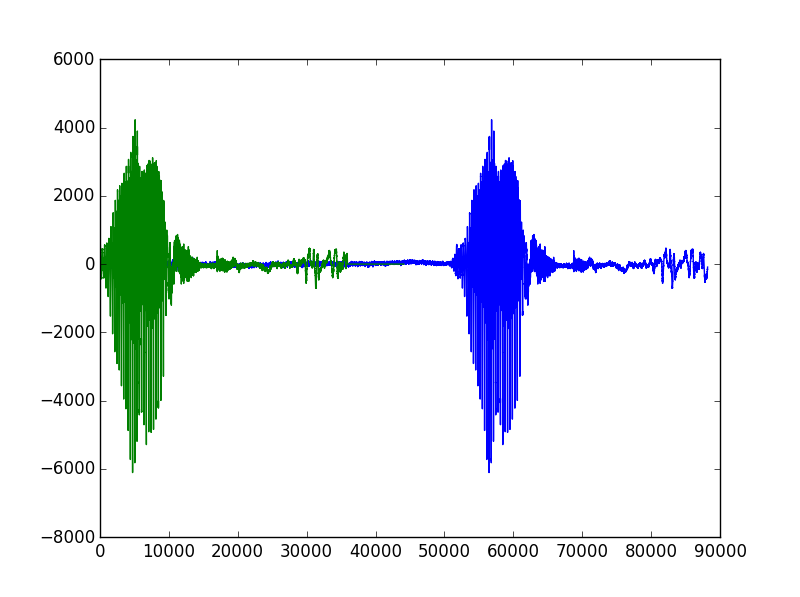
\includegraphics[width=\textwidth]{media/triggertest.png}
\label{fig:Wurst_Triggered}
\caption{Das Wort 'Wurst' in der Zeitdomäne.}
\end{figure}

\begin{figure}[H]
\label{fig:Wurst_Fourier}
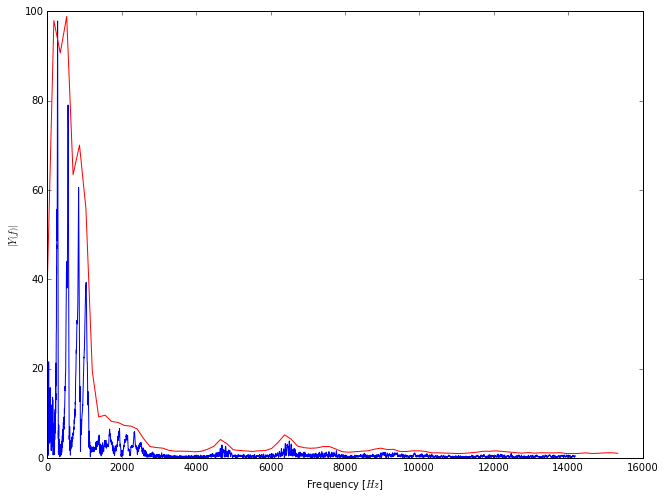
\includegraphics[width=\textwidth]{media/Wurst_vgl.png}
\caption{Das Wort 'Wurst' in der Frequenzdomäne}
\end{figure}


\section{Auswertung und Interpretation}
\label{chap:VERSUCH_1_AUSWERTUNG}
In Abbildung \ref{fig:Wurst_Triggered} ist ein Beispielhaftes Signal in der Zeitdomäne zu sehen. Der Blaue Signalverlauf ist das Signal ohne Triggerung. Der Grüne Graph ergibt sich aus dem blauen Signal nach Triggerung und Zuschnitt auf eine Sekunde. Die X-Achse stellt wie zu erwarten die Zeit in Sekunden dar. Die Einheit des Wertebereichs ist schwierig zu deuten, da den Versuchsdurchführenden nicht bekannt ist, was für Werte die Soundkarte zurückliefert. Das Ergebnis entspricht also den Erwartungen. Für dieses Beispielhafte Signal ist in Abbildung \ref{fig:Wurst_Fourier} das Spektrum zu sehen. Die Blauen linien sind das Spektrum ohne Windowing. Die Rote Line ist das Spektrum mit Windowing.
Bei diesem gilt selbiges für den Wertebereich, wie bei dem Signal im Zeitbereich. 
Die in diesem Versuch implementierten Funktionen werden im folgenden für die Implementierung des Spracherkenners benutzt.
